
% Attention, il faut déclarer la librairie calc :\usetikzlibrary{calc}  pour les calculs de coordonnées des points


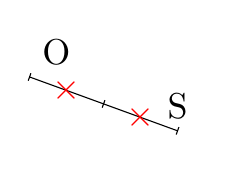
\begin{tikzpicture}	[scale=0.5,every node/.style={scale=1.3}]

\begin{scope}[rotate=-20] %la figure
\draw (-2,0)--(0,0) node [midway,red] {$\times$};
\draw (0,0)--(2,0) node [midway,red] {$\times$};
\draw (-2,0)--+(90:0.1)--+(-90:0.1);
\draw (2,0)--+(90:0.1)--+(-90:0.1);
\draw (0,0)--+(90:0.1)--+(-90:0.1);
\node [above right] at (-2,0) {O};
\node [above] at (2,0) {S};
\end{scope}

\end{tikzpicture} 
 
